%-------------------------------------------------------------------------
\newpage
\section{Deformation processes}
\label{sec:def_proc}

\subsection{Kinematics of deformation processes}
\label{sec:kinematics}

Kinematics analyzes the geometry of motion in general, and of deformation processes in particular. It is based on the assumption that a material (physical) body $\mathcal{B}$, which represents a set of elements $\mathcal{P}$ called material points (aka: material elements, particles), at each moment of time can be uniquely defined with certain parts (usually different if motion occurs) of space. Assigning the material body particularly to its image in the three-dimensional Euclidean space of physical observations, the location of each material point at each time can be identified with the position vector $\mathbf{x}(t)$ in a physically well-founded manner. Consequently, the position vector can be represented by its Cartesian coordinates $x_1,\,x_2,\,x_3$. In order to characterize the motion of a material body uniquely with respect to a reference state, the domain in space occupied by the material body at an arbitrarily selected time $t_0$ is of an emphasized significance. Usually in porous media mechanics, an appropriately chosen initial state of the solid skeleton is chosen as the reference state. The position vectors to define the positions of the material points at $t_0$ are denoted as $\mathbf{X}$.

\begin{figure}[htb!]
\begin{center}
\footnotesize
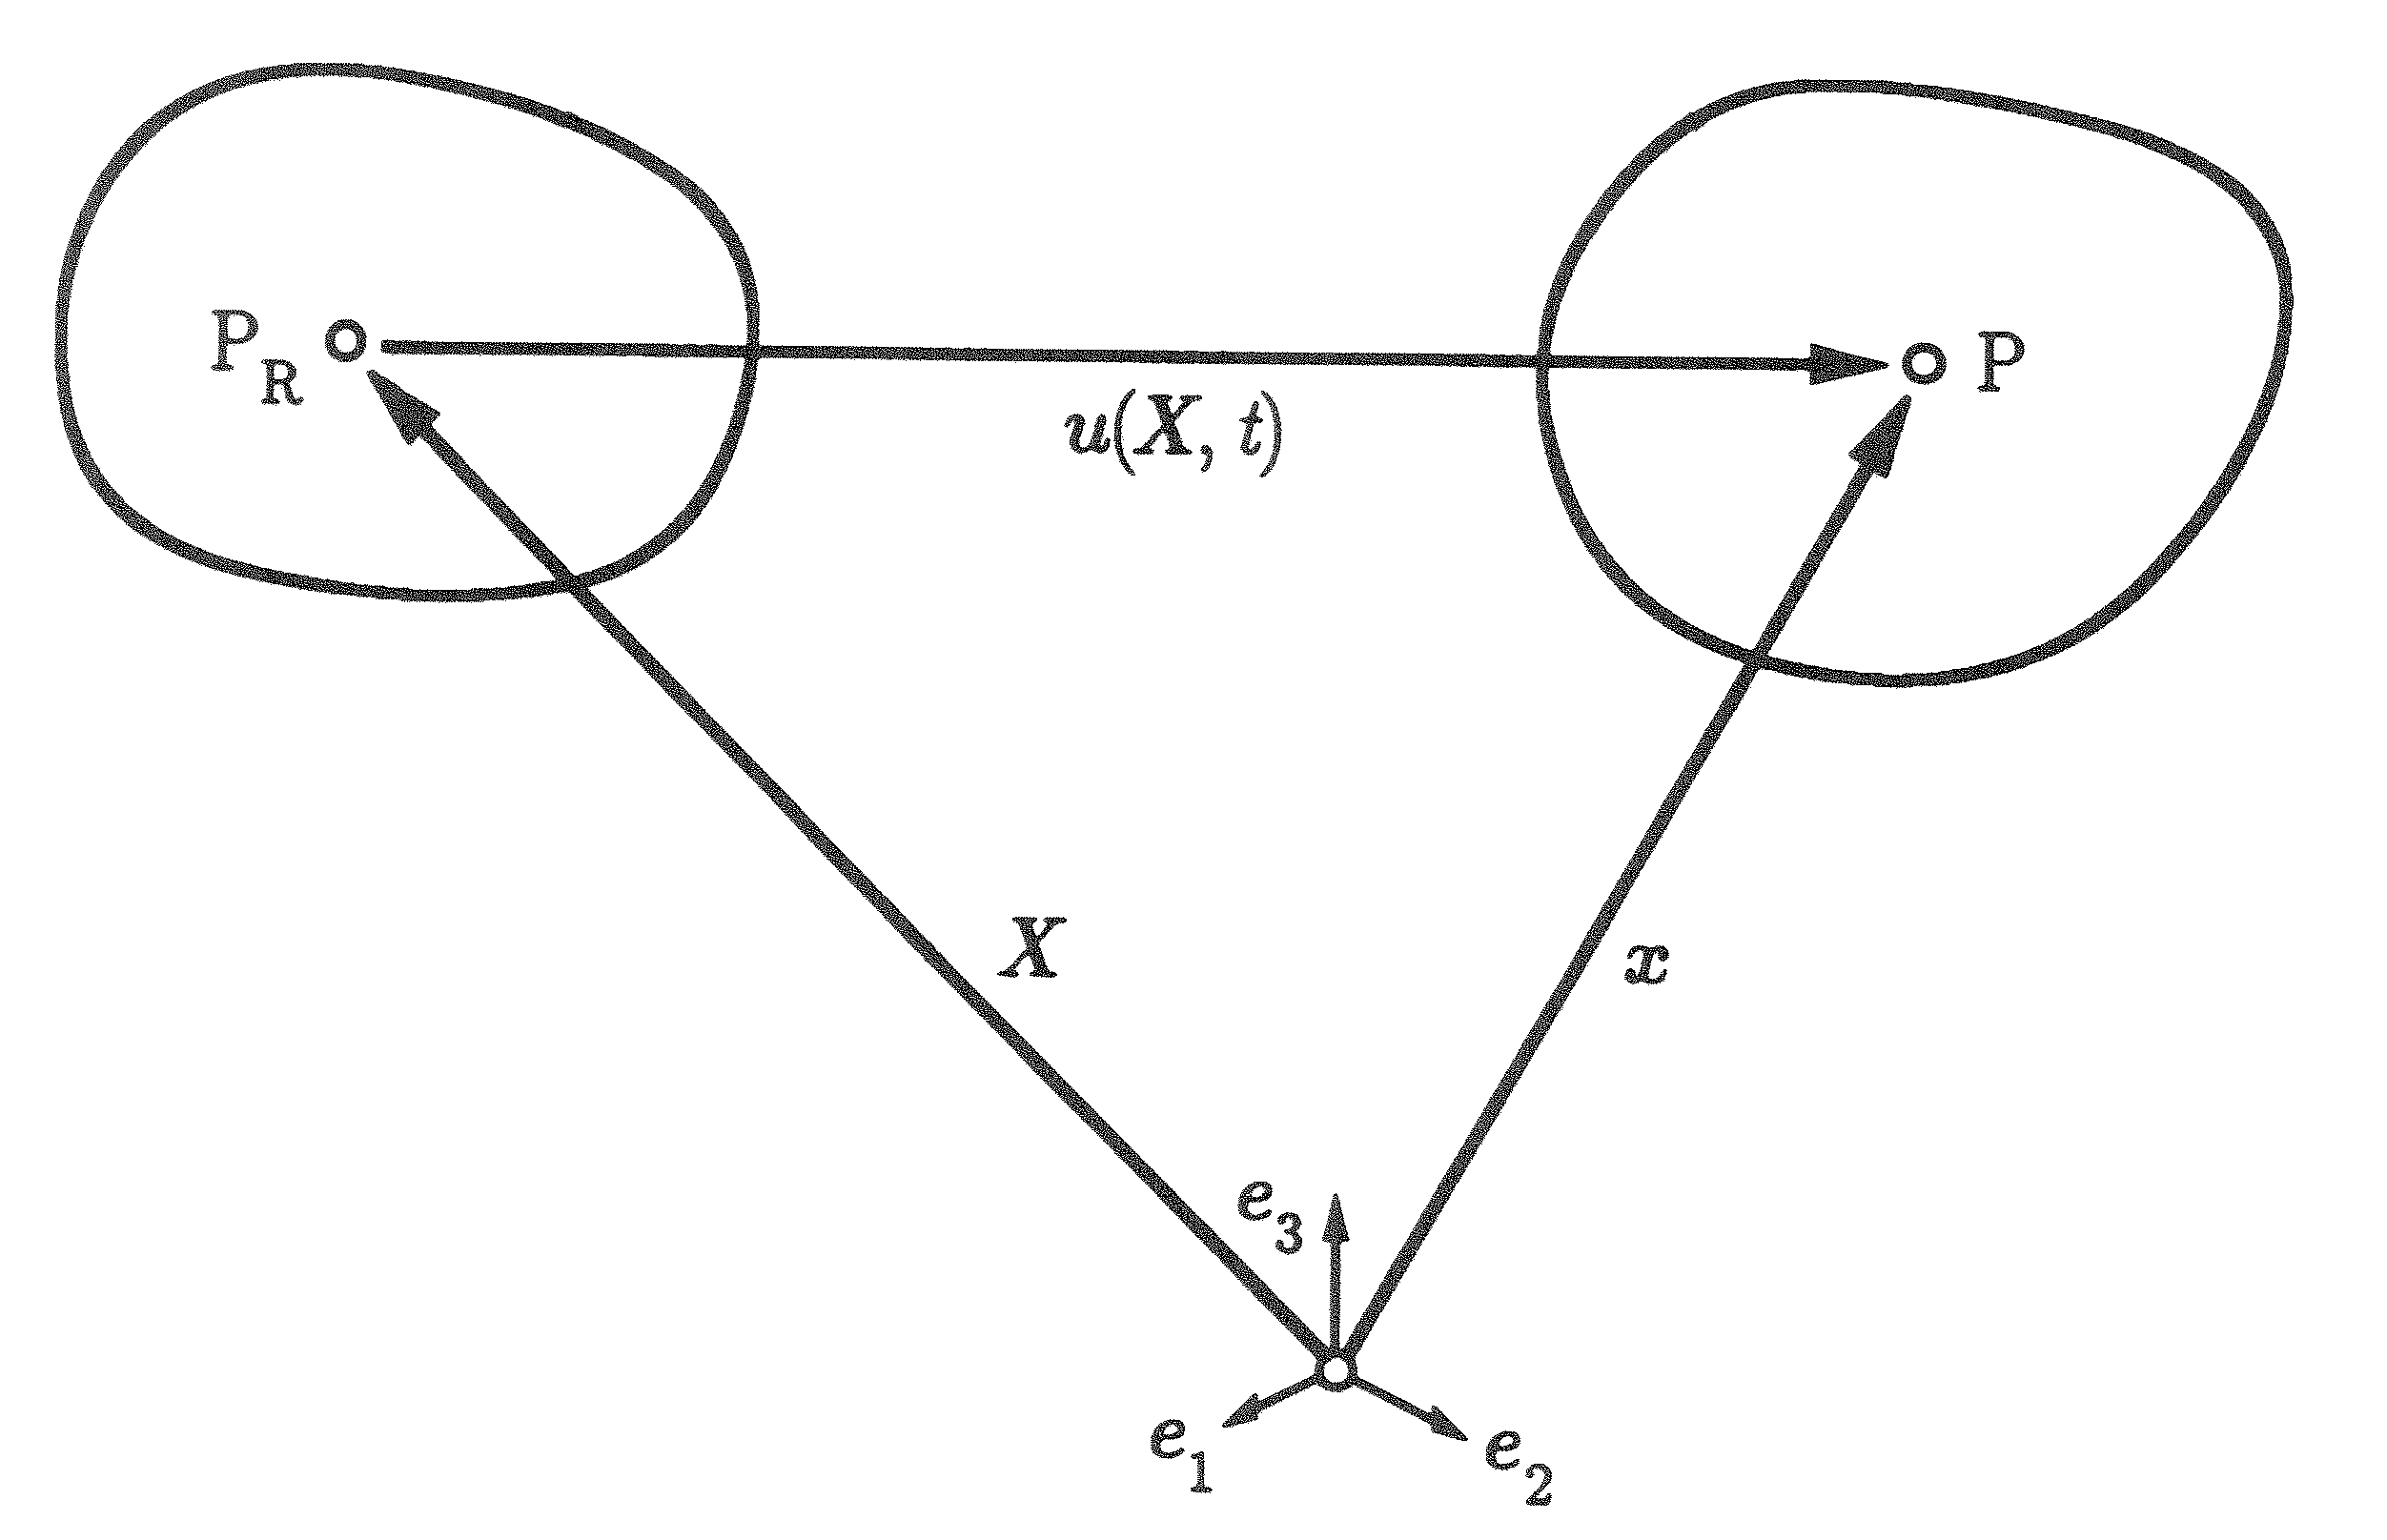
\includegraphics[width=0.7\textwidth]{figures/disp_vect.eps}
\caption{Definition of the displacement vector as the difference of the position vectors $\mathbf{x}$ and $\mathbf{X}$ of a material point (particle) of the body under consideration at various time $t$ (current time) and $t_0$ (Haupt, 2002 \cite{Haupt:2002})}
\label{fig:disp_vect}
\end{center}
\end{figure}

One of the primary variables within the context of the numerical simulation of coupled THM processes is the displacement vector $\mathbf{u}$ of the solid phase. The displacement vector is a commonly used kinematic variable to describe the motion (rigid body motion and/or deformation) of a solid material, and quantifies the change in the position of a given material point (cf. Fig.~\ref{fig:disp_vect}).
\begin{equation}
\mathbf{u}(\mathbf{X},t)\,=\,\mathbf{x}(\mathbf{X},t)\,-\,\mathbf{X}
\label{eq:defvec}
\end{equation}
In other words: the displacement vector connects the current position $\mathbf{x}$ of a material point which under the impact of external forces has been moved, and was located at time $t_0$ at the position $\mathbf{X}$. As, in general, the displacement vector will vary locally and temporally, $\mathbf{u}(\mathbf{X},t)=\mathbf{u}(\mathbf{X}(\mathbf{x},t),t)=\bar{\mathbf{u}}(\mathbf{x}{}{},t)\equiv\mathbf{u}$ represents a vector field as function of space and time.

For the sake of the possible comparison of the response of material bodies, which are composed of different materials and/or have a different geometry, to the impact of external forces it is not reasonable to deal with the physically obvious variables displacement and force, but rather to introduce relative physical variables like strain and stress measures. Strain measures represent second-order kinematic tensor variables characterizing the local deformation processes, which deviate from the rigid body motion of a material body.

Based on the definition of the displacement gradient
\begin{equation}
\nabla{\bar{\mathbf{u}}}(\mathbf{x},t)\,=\,\frac{\partial u_i}{\partial x_j}\,\miu{e}{i}{}\otimes\miu{e}{j}{}
\label{eq:dispgrad}
\end{equation}
with the orthonormal system of Cartesian base vectors $\miu{e}{i}{}$ ($i=1,2,3$), the strain tensor $\miu{\varepsilon}{}{}(\mathbf{x},t)$ in case of small (infinitesimal) deformations is established as the symmetric part of the displacement gradient.
\begin{equation}
\miu{\varepsilon}{}{}(\mathbf{x},t)\,=\,\frac{1}{2}
\left(\nabla{\bar{\mathbf{u}}}(\mathbf{x},t)\,+\,\left(\nabla{\bar{\mathbf{u}}}(\mathbf{x},t)\right)^{\mathrm{T}}\right)
\label{eq:straintens}
\end{equation}

The matrix of the coefficients of the strain tensor consists of so-called normal components
\begin{equation}
\varepsilon_{ii}\,=\,\frac{\partial u_i}{\partial x_i}
\label{eq:straintensnormal}
\end{equation}
and shear components.
\begin{equation}
\varepsilon_{ij}\,=\,
\frac{1}{2}\left(\frac{\partial u_i}{\partial x_j}\,+\,\frac{\partial u_j}{\partial x_i}\right)
\qquad(i\neq{j})
\label{eq:straintensshear}
\end{equation}
For special cases it can be easily shown that normal strain is geometrically interpreted as elongation of material line elements (cf. Fig.~\ref{fig:extension}),
\begin{figure}[htb!]
\begin{center}
\footnotesize
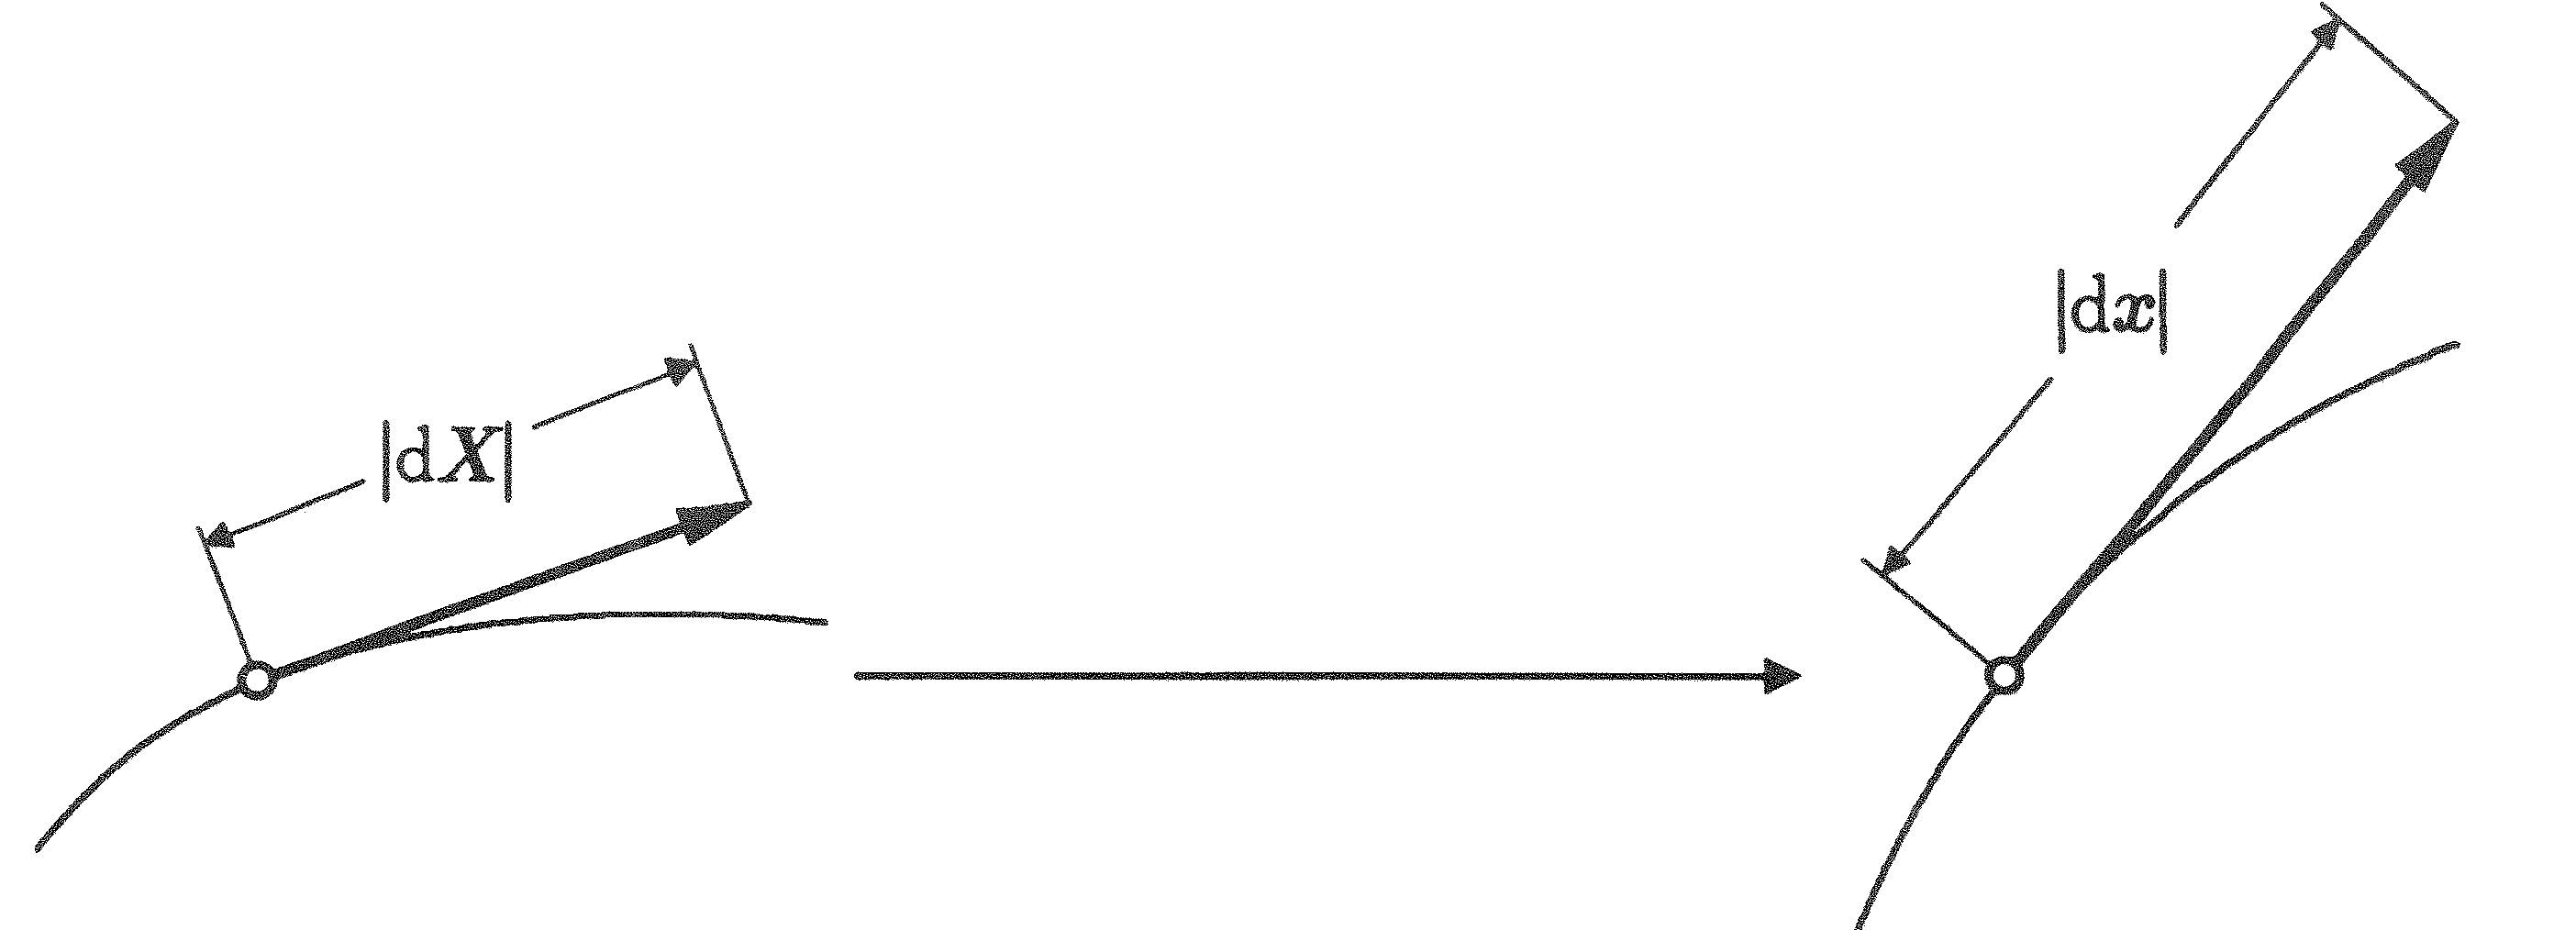
\includegraphics[width=0.7\textwidth]{figures/extension.eps}
\caption{Extension (normal strain) of a material line element $d\mathbf{X}=\vert d\mathbf{X}\vert\miu{e}{}{}$
(Haupt, 2002 \cite{Haupt:2002})}
\label{fig:extension}
\end{center}
\end{figure}

and shear strain represents the change of the angle between two material line elements, which initially were perpendicular to each other (cf. Fig.~\ref{fig:shear}).
\begin{figure}[htb!]
\begin{center}
\footnotesize
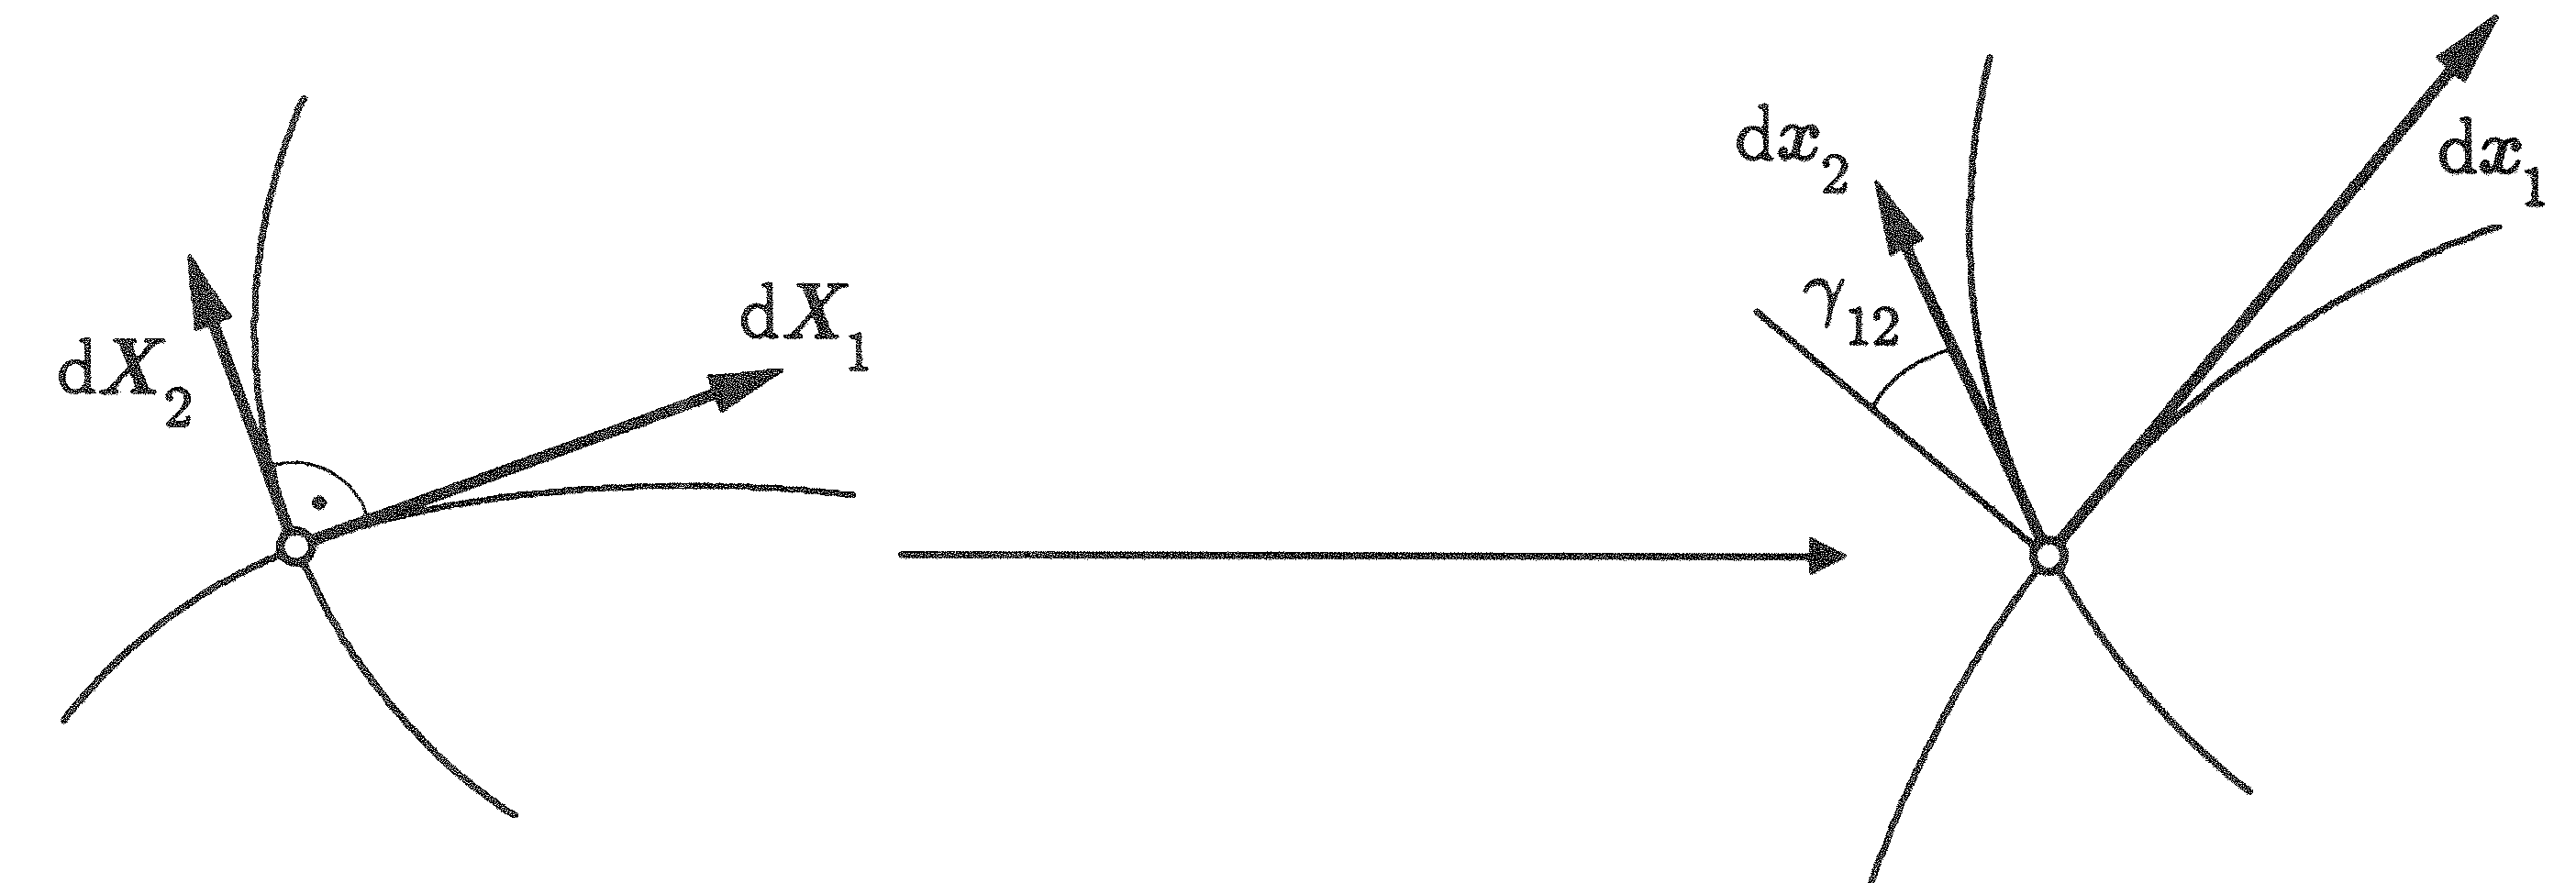
\includegraphics[width=0.7\textwidth]{figures/shear.eps}
\caption{Shear (shear strain) of two material line elements $d\mathbf{X}_1=\vert d\mathbf{X}_1\vert\miu{e}{1}{}$ and $d\mathbf{X}_2=\vert d\mathbf{X}_2\vert\miu{e}{2}{}$, which are orthogonal in the undeformed state (Haupt, 2002 \cite{Haupt:2002})}
\label{fig:shear}
\end{center}
\end{figure}

For the analysis of certain deformation processes it is reasonable to consider local volume changes and shape changes separately. Within this context, the strain tensor can be additively split into two parts: a volumetric $\miu{\varepsilon}{v}{}$ and a so-called deviatoric (volume-preserving) $\miu{\varepsilon}{d}{}$ one.
\begin{equation}
\miu{\varepsilon}{}{}\,=\,\miu{\varepsilon}{d}{}\,+\,\miu{\varepsilon}{v}{}
\label{eq:strainsplit}
\end{equation}
The individual partial strain tensors are defined as follows:
\begin{eqnarray}
\miu{\varepsilon}{v}{} & = & \frac{1}{3}\mathrm{tr}(\miu{\varepsilon}{}{})\,\mathbf{I}\,=\,
\frac{1}{3}(\varepsilon_{11}+\varepsilon_{22}+\varepsilon_{33})\,\mathbf{I}
\label{eq:devstrain}
 \\[2.0ex]
\miu{\varepsilon}{d}{} & = & \miu{\varepsilon}{}{}\,-\,\miu{\varepsilon}{v}{}
\label{eq:volstrain}
\end{eqnarray}

Based on the definition
\begin{equation}
\mathbf{v}^s(\mathbf{x},t)\,=\,\mathop{\bar{\mathbf{u}}}\limits^{\miu{.}{}{}}(\mathbf{x},t)
\label{eq:solidveloc}
\end{equation}
of the velocity of material points of the solid skeleton, the strain rate tensor
\begin{equation}
\miu{\varepsilon}{}{\dot}(\mathbf{x},t)\,=\,\mathbf{d}(\mathbf{x},t)\,=\,\frac{1}{2}
\left(\nabla\mathbf{v}^s(\mathbf{x},t)\,+\,\left(\nabla\mathbf{v}^s(\mathbf{x},t)\right)^{\mathrm{T}}\right)
\label{eq:strainratetens}
\end{equation}
with its coefficients
\begin{equation}
d_{ij}\,=\,
\frac{1}{2}\left(\frac{\partial v^s_i}{\partial x_j}\,+\,\frac{\partial v^s_j}{\partial x_i}\right)
\label{eq:strainratecoeff}
\end{equation}
can be defined, which is necessary for the investigation of deformation processes in case of rate-dependent material behavior.

In case of small strains, which was assumed here, the relation between the strain tensor and the displacement vector is a linear one (see. (\ref{eq:straintens})). Considering large strains, the definition of appropriate strain measures requires more sophisticated reflections about the kinematcs of motion. As a result, different strain tensors can be obtained representing non-linear functions of the displacement vector. 

%-------------------------------------------------------------------------
\newpage
\subsection{Stress Tensor}
\label{sec:stresstensor}

The momentum as well as the moment of momentum of a material body are affected by external forces acting on it, which represent the mechanical effect of the surroundings (cf. Fig.~\ref{fig:ext_forces}). Summarizing all local forces, the resultant force $\mathcal{F}$ can be defined.
\begin{equation}
\mathcal{F}\,=\,
\int\limits_{\partial\mathcal{B}}\mathbf{t}\,da\,+\,\int\limits_{\mathcal{B}}\mathbf{f}\,dm\,=\,
\int\limits_{\Gamma}\mathbf{t}(\mathbf{x},t,\mathbf{n})\,d\Gamma\,+\,
\int\limits_{\Omega}\mathbf{f}_v(\mathbf{x},t)\,\varrho(\mathbf{x},t)\,d\Omega
\label{eq:result_force}
\end{equation}
Generally, the material body under consideration bears forces distributed over its surface with the surface force
density $\mathbf{t}$ (traction, Cauchy stress vector), and forces distributed over the volume of the material body with the volume force density (mass distributed specific volume force) $\mathbf{f}_v$. As mentioned above, only gravity $\varrho\mathbf{g}$ should be considered as specific volume force.

\begin{figure}[htb!]
\begin{center}
\footnotesize
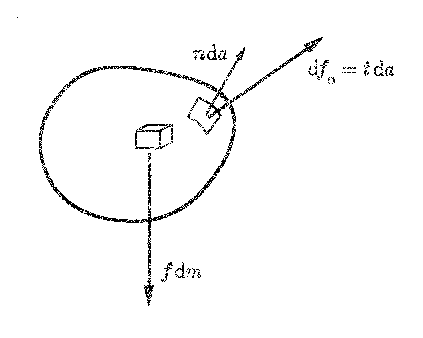
\includegraphics[width=0.6\textwidth]{figures/ext_forces.eps}
\caption{External volume and surface forces acting on infinitesimal geometrical elements of a material body (Haupt, 2002 \cite{Haupt:2002})}
\label{fig:ext_forces}
\end{center}
\end{figure}

The traction vector $\mathbf{t}(\mathbf{x},t,\mathbf{n})$ is considered to be a function of the location of its action on the surface, a function of time and of the normal vector, which characterizes the orientation of the surface element $d\miu{\Gamma}{}{}$. Assuming a linear relation between the traction and the normal vector (Cauchy's theorem), the stress measure $\miu{\sigma}{}{}(\mathbf{x},t)$ (Cauchy stress tensor) is defined as a link between surface traction and surface orientation. 
\begin{equation}
\mathbf{t}(\mathbf{x},t,\mathbf{n})\,=\,\miu{\sigma}{}{}(\mathbf{x},t)\,\mathbf{n}
\qquad\Rightarrow\qquad
\miu{\sigma}{}{}\,=\,\sigma_{ij}\,\miu{e}{i}{}\otimes\miu{e}{j}{}
\label{eq:cauchy_theorem}
\end{equation}
Based on Cauchy's theorem, the differential surface force $d\mathbf{f}_0$ acting on a surface element can be obtained. 
\begin{equation}
d\mathbf{f}_0\,=\,\mathbf{t}\,d\Gamma\,=\,(\miu{\sigma}{}{}\,\mathbf{n})\,d\Gamma\,=\,
\miu{\sigma}{}{}\,(\mathbf{n}\,d\Gamma)\,=\,\miu{\sigma}{}{}\,d\miu{\Gamma}{}{}
\label{eq:differ_surforce}
\end{equation}

For certain cases it is reasonable to use the so-called Kirchhoff stress tensor $\miu{\tau}{}{}$, a weighted Cauchy stress measure, instead of the Cauchy stress tensor itself.
\begin{equation}
\miu{\tau}{}{}\,=\,\frac{\varrho_0}{\varrho}\,\miu{\sigma}{}{}
\end{equation}

The second-order stress tensor characterizes the local internal load state referring to a material point of the body under consideration. Generally, it can be defined by three stress vectors acting on three faces of an infinitesimal tetrahedron, which are perpendicular to each other analyzing the equilibrium of forces for this domain. The coefficients of the resulting stress tensor are denoted by two indices -- the first indicates the direction of the normal vector of the face under consideration, the second one the direction of the stress coefficient (see Fig.~\ref{fig:stresstens_plane} for the two-dimensional case, extension to the three-dimensional case is straightforward).

%\begin{figure}[htb!]
%\begin{center}
%\footnotesize
%\includegraphics[width=0.6\textwidth]{figures/cauchy_law.png}
%\caption{Equilibrium of surface tractions acting on the edges of an infinitesimal triangular element. Definition of %the Cauchy stress tensor using Cauchy's theorem (Jaeger et al. \cite{JCZ:2007})}
%\label{fig:cauchy_law}
%\end{center}
%\end{figure}

\begin{figure}[htb!]
\begin{center}
\footnotesize
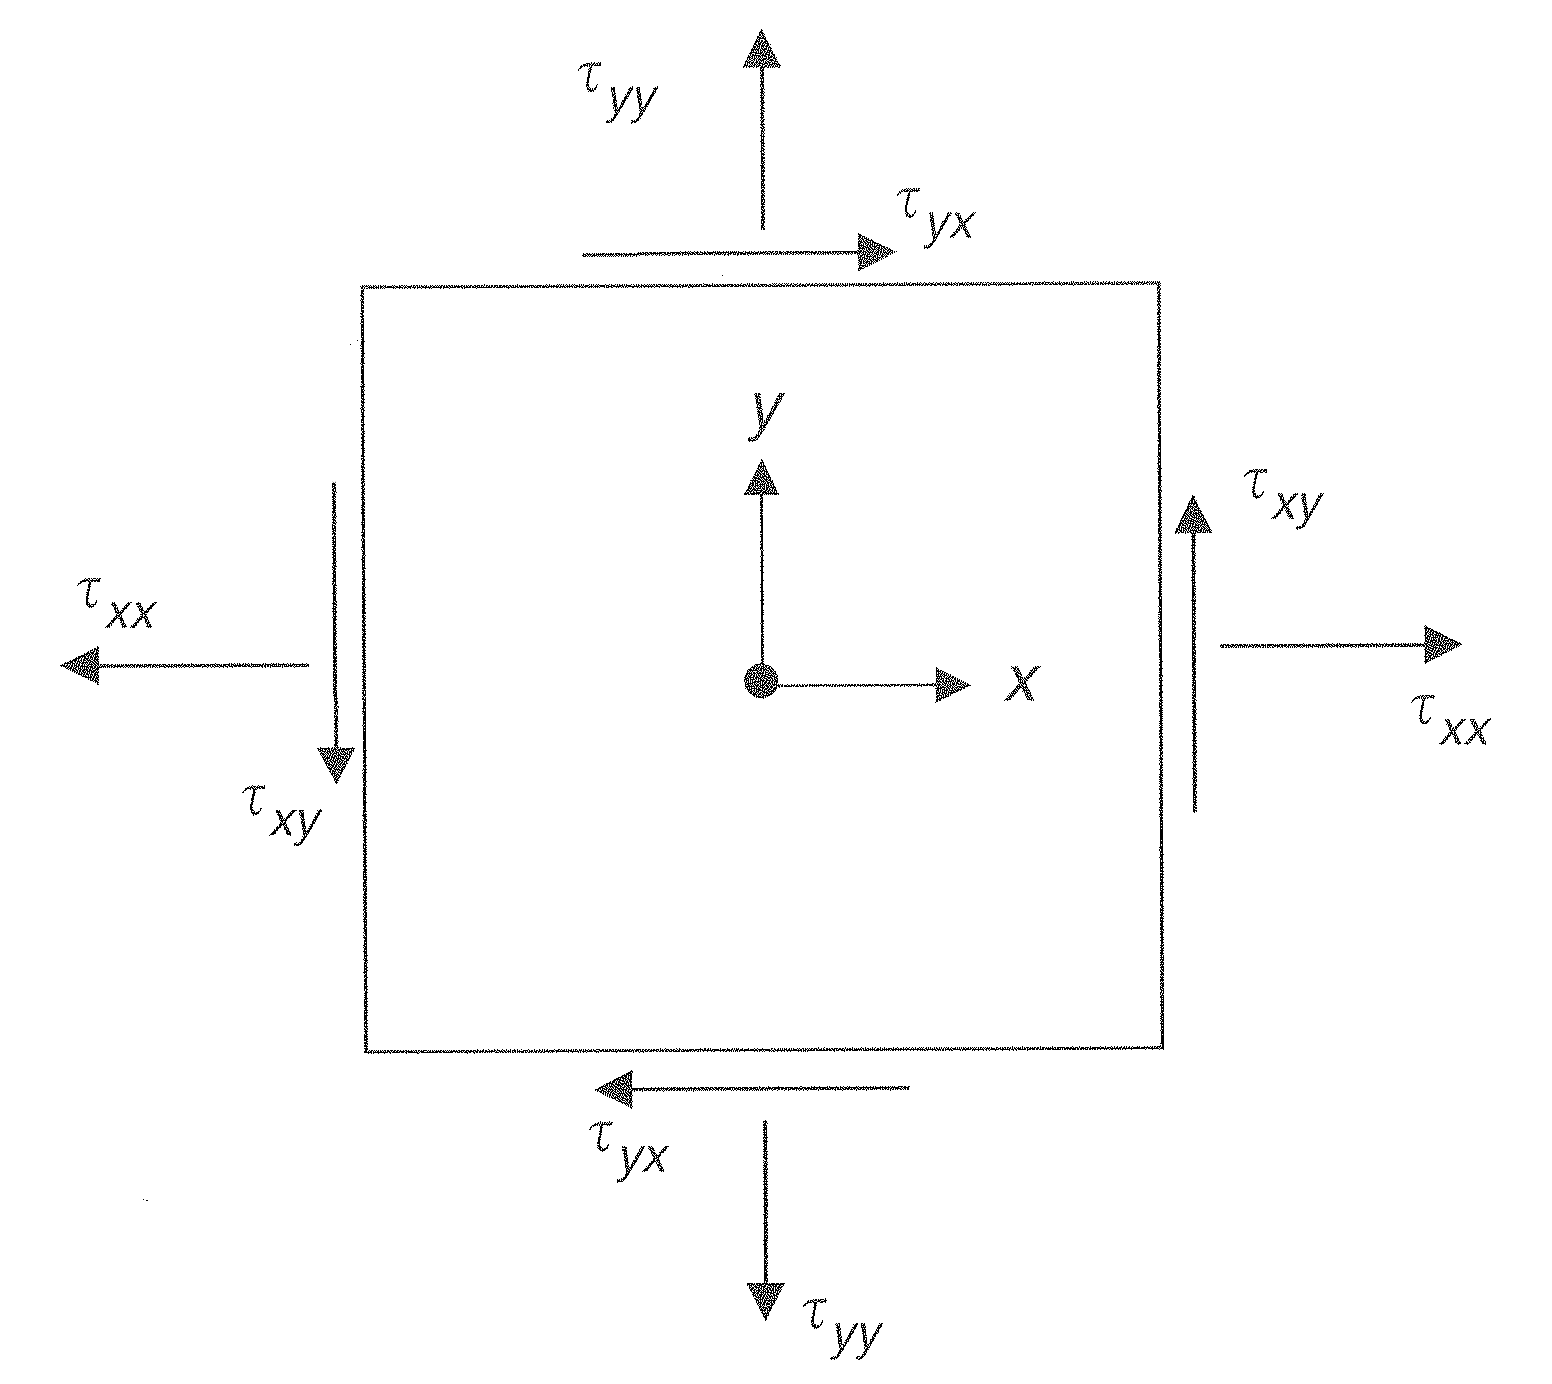
\includegraphics[width=0.6\textwidth]{figures/stresstens_plane.eps}
\caption{Coefficients of the stress tensor acting on a small plane quadrilateral element (Jaeger et al. \cite{JCZ:2007})}
\label{fig:stresstens_plane}
\end{center}
\end{figure}

The sign convention, usually applied in continuum mechanics, implies positive stress coefficients coinciding with the directions of the axes of coordinates at faces with normal vectors also coinciding with the directions of the axes of ccordinates. Consequently, tensile stress coefficients are positive, compressive stresses negative. Positive stress coefficients on opposite faces are oppositely directed (but of equal absolute value). The matrix of the coefficients of the (Kirchhoff) stress tensor is composed as follows:
\begin{equation}
\tau_{ij}\,=\,
\left(
\begin{array}{ccc}
\tau_{xx} & \tau_{xy} & \tau_{xz} \\
\tau_{yx} & \tau_{yy} & \tau_{yz} \\
\tau_{zx} & \tau_{zy} & \tau_{zz}
\end{array}
\right)
\label{eq:stress_matrix}
\end{equation}
Analogous to the strain tensor, the coefficients $\tau_{xx},\,\tau_{yy},\,\tau_{zz}$ are called normal stresses, the coefficients $\tau_{ij}\quad(i\neq j)$ shear stresses with $\tau_{ij}=\tau_{ji}$ (symmetry of the stress tensor, which results from the balance of moment of momentum).

In the special uniaxial stress case only at one face of a volume element a normal stress occurs, whereas all the other faces are stress-free. Consequently, the stress coefficient is calculated as the force acting on the face under consideration divided by its area.
